\documentclass[conference]{IEEEtran}
\IEEEoverridecommandlockouts
\usepackage{cite}
\usepackage{amsmath,amssymb,amsfonts}
\usepackage{algorithmic}
\usepackage{algorithm}
\usepackage{graphicx}
\usepackage{textcomp}
\usepackage{xcolor}
\usepackage{booktabs}
\usepackage{multirow}
\usepackage{hyperref}


\def\BibTeX{{\rm B\kern-.05em{\sc i\kern-.025em b}\kern-.08em
    T\kern-.1667em\lower.7ex\hbox{E}\kern-.125emX}}

\begin{document}

\title{CUDA-Accelerated Multi-Layer Perceptron for MNIST Using Two-Phase Gradient Accumulation}

\author{
\IEEEauthorblockN{Samartha H V}
\IEEEauthorblockA{\textit{Manipal Institute of Technology Bengaluru} \\
\textit{Manipal Academy of Higher Education} \\
Manipal, India \\
samartha1.mitblr2025@learner.manipal.edu}
\and
\IEEEauthorblockN{Chiranth R}
\IEEEauthorblockA{\textit{Manipal Institute of Technology Bengaluru} \\
\textit{Manipal Academy of Higher Education} \\
Manipal, India \\
chiranth1.mitblr2025@learner.manipal.edu}
}


\maketitle

\begin{abstract}
Training neural networks on CPUs has always been frustratingly slow, which is what motivated us to explore GPU acceleration for this project. In this work, we implemented a GPU-accelerated Multi-Layer Perceptron (MLP) from scratch using CUDA for the classic MNIST digit classification task. What started as a straightforward parallelization effort quickly revealed some interesting challenges—particularly race conditions in optimizer implementations that we hadn't anticipated. We ended up developing a two-phase gradient accumulation approach that fixed these issues and enabled Momentum and Adam optimizations to work correctly on the GPU. Performance gains were quite significant: our CUDA implementation runs 100-202× faster than the serial CPU version, completing training epochs in under half a second compared to about 90 seconds on the CPU. We tested three different optimizers (SGD, Momentum and Adam) and found that Adam not only achieved the best accuracy (80.8\% in 20 epochs) but was also the fastest to train—somewhat counterintuitively given its computational overhead. We also experimented with shared memory optimizations that provided an additional 6.5-15.8\% speedup. The final system includes model saving/loading functionality and a standalone GPU inference program that can classify images in 0.4 milliseconds, processing around 2,500 images per second.
\end{abstract}

\begin{IEEEkeywords}
CUDA, GPU Acceleration, Neural Networks, Deep Learning, MNIST, Parallel Processing, High-Performance Computing, Backpropagation, Optimization Algorithms
\end{IEEEkeywords}


\section{Introduction}

Training neural networks is often a computationally intensive process, particularly when relying solely on CPU-based implementations. During the early stages of our coursework and experimentation with neural networks, one of the most challenging aspects was the extended time required for training models. Even when using relatively small datasets, CPU training often took several hours, and it was evident that this problem would only worsen as network architectures became larger and more complex. This observation motivated our exploration of GPU acceleration as part of our M.Tech project, with the goal of significantly improving training efficiency without compromising model accuracy.

Graphics Processing Units (GPUs) offer a fundamentally different computational paradigm compared to Central Processing Units (CPUs). While CPUs are designed with a limited number of powerful cores optimized for sequential execution, GPUs consist of thousands of lightweight cores capable of executing numerous parallel operations simultaneously. This parallel architecture makes GPUs particularly well-suited for neural network training, where identical mathematical operations are repeatedly applied across large sets of data. Using this property enables substantial reductions in training time and computational overhead.

To investigate the impact of GPU acceleration, we focused on the MNIST dataset—a classic benchmark for handwritten digit recognition that consists of 60,000 training images and 10,000 test images, each of size 28×28 pixels, resulting in 784 input features when flattened. Although MNIST is relatively simple compared to modern large-scale datasets such as ImageNet, it provides an excellent starting point for understanding the core principles of GPU-accelerated training. The techniques developed in this study can easily be extended to more complex datasets and deeper architectures.

The primary objective of this work was to design and implement a complete CUDA-based multilayer perceptron (MLP) framework capable of achieving significant computational speedup—ranging from 100× to 200×—over CPU-based implementations, while maintaining comparable accuracy. Additionally, we aimed to systematically explore different optimization strategies, both at the low-level (such as the use of shared memory in CUDA kernels) and high-level (including optimizer selection among SGD, Momentum, and Adam). Another important goal was to build an end-to-end system that not only enables efficient training, but also supports model saving and provides high-speed inference, making it practical for real-world deployment.

Through this research, several key contributions were made. We developed a fully functional CUDA-based MLP training system that supports multiple hidden layers and various architectural configurations. During the development process, we identified and resolved a critical race condition that affected the Momentum and Adam optimizers, caused by improper parallelization of optimizer state updates. To address this, we introduced a two-phase gradient accumulation strategy that ensured correct and consistent updates, a technique that may prove useful for other parallelized implementations. Comprehensive benchmarking was conducted to evaluate the effects of batch size, optimizer choice, and network depth on both performance and accuracy. Our results revealed that Adam optimizer not only produced the highest classification accuracy of 80.8\% but also achieved the fastest training speed, with an average of 0.445 seconds per epoch, despite performing more computations per iteration. Furthermore, we implemented a standalone GPU inference module capable of classifying images in under one millisecond (0.4 ms per image), demonstrating the system’s efficiency and real-world applicability. Overall, the outcomes of this work highlight the significant advantages of GPU acceleration in neural network training and provide valuable insights into the design of efficient, scalable deep learning systems.

\section{Literature Review}

Author Wang et al. [4] developed a GPU-accelerated inference framework for scientific computing applications and achieved a 17× speedup by applying optimized batching strategies. The study highlighted the significance of batch management for maximizing GPU utilization but was limited in scalability across diverse neural network architectures. In [5], Rao et al. proposed a CUDA-based deep neural network training method that accelerated backpropagation by up to 487× compared to CPU training. However, their model required extensive manual kernel tuning and lacked flexibility for different network sizes, making it less generalizable.

Ramroach et al. [6] implemented CUDA-optimized neural networks for biomedical data prediction, demonstrating a 65× computational speedup. Despite its efficiency, the approach suffered from GPU memory bandwidth constraints and limited applicability to large-scale models. Huang et al. [11] introduced a Tensor Core-aware pruning method that achieved faster inference using hardware-optimized matrix multiplication, reaching high accuracy but remaining hardware-specific. Similarly, Li et al. [12] proposed GPU memory access optimizations to improve throughput in deep learning workloads. Although their results showed clear performance improvements, the focus was limited to memory analysis and lacked end-to-end training validation.

LeCun et al. [1] introduced the MNIST dataset, which has become a foundational benchmark for handwritten digit recognition. Nielsen [3] discussed theoretical perspectives on neural network learning and emphasized the importance of activation functions for efficient convergence. Bengio [9] offered practical recommendations for gradient-based optimization in deep networks, highlighting how hyperparameter tuning influences stability. Kingma and Ba [7] proposed the Adam optimizer, which combined adaptive learning rates with momentum, and has since become a standard for deep learning optimization. Ioffe and Szegedy [8] introduced Batch Normalization to mitigate internal covariate shift, which significantly improved convergence but remained difficult to parallelize efficiently on GPUs.

Dean et al. [10] developed a large-scale distributed training framework for deep neural networks that addressed communication bottlenecks using asynchronous gradient updates. Although this work focused on CPU-based distributed environments, its findings inspired later GPU-oriented parallelization studies. Kim and Park [13] extended this idea by implementing distributed stochastic gradient descent across multiple GPUs, achieving up to 2.5× faster convergence. However, the model faced communication delays between GPUs. Zhao et al. [14] presented a CUDA-accelerated backpropagation model for MNIST, achieving 97.2\% accuracy with a 110× training speedup, though kernel synchronization overhead limited performance scaling.

Xu et al. [15] introduced mixed-precision training techniques using FP16 arithmetic, which reduced computation time by 1.8× while maintaining comparable accuracy. The method, however, introduced minor instability in early training epochs. Zhang et al. [16] proposed a dynamic memory allocation and CUDA stream overlap approach, which improved throughput but increased implementation complexity. Huang and Patel [17] introduced kernel fusion techniques to reduce synchronization latency, resulting in 30–40\% faster training on CNNs, though benefits diminished for smaller networks.

Luo et al. [18] investigated atomic operation overheads in GPU-based gradient updates and proposed a fine-grained synchronization mechanism to reduce contention in shared memory. The method improved consistency but slightly increased latency due to additional synchronization. Tan and Chen [19] designed a hybrid CPU–GPU deep learning framework to minimize PCIe data transfer overhead, achieving a 2.3× acceleration but suffering from limited scalability for real-time applications. Akhtar et al. [20] presented a low-level CUDA optimization technique involving shared memory tiling and register blocking, improving performance by 10–20\%, but with considerable kernel design complexity.

From the reviewed literature, it is evident that GPU acceleration, memory optimization, and parallelized backpropagation have substantially advanced neural network training efficiency. Nevertheless, few studies have presented complete from-scratch CUDA implementations that explicitly address race conditions in stateful optimizers such as Momentum and Adam. This research aims to fill that gap by developing a robust CUDA-based MLP framework using a two-phase gradient accumulation mechanism that ensures correctness, stability, and high performance during parallel training.

\section{Methodology}

\subsection{Neural Network Architecture}

Our MLP architecture is fairly standard: we have an input layer with 784 neurons (one for each pixel in the flattened 28×28 images), one or more hidden layers with a configurable number of neurons (we used 128 in most experiments), and an output layer with 10 neurons for the digit classes.

The forward pass through each layer is just an affine transformation followed by an activation function:
\begin{equation}
a^{(l)} = \text{activation}(W^{(l)} a^{(l-1)} + b^{(l)})
\end{equation}

We went with ReLU activation for the hidden layers because it's simple and works well, and softmax for the output layer to get probability distributions over the 10 digit classes. For the loss function, we used standard cross-entropy:

\begin{equation}
\mathcal{L} = -\frac{1}{N} \sum_{i=1}^{N} \log(\hat{y}_{i,c_i})
\end{equation}
where $c_i$ is the index of the correct class for sample $i$.
The forward propagation for each layer can be expressed as:
\begin{equation}
z^{(l)} = W^{(l)} a^{(l-1)} + b^{(l)}, \quad a^{(l)} = f(z^{(l)})
\end{equation}

where $W^{(l)}$ and $b^{(l)}$ denote the weight matrix and bias vector for layer $l$, $a^{(l-1)}$ is the activation from the previous layer, and $f(\cdot)$ is the activation function (ReLU in this case).

During backpropagation, the gradients are computed as follows:
\begin{equation}
\delta^{(l)} = (W^{(l+1)})^T \delta^{(l+1)} \odot f'(z^{(l)})
\end{equation}

\begin{equation}
\frac{\partial \mathcal{L}}{\partial W^{(l)}} = \delta^{(l)} (a^{(l-1)})^T, \quad
\frac{\partial \mathcal{L}}{\partial b^{(l)}} = \delta^{(l)}
\end{equation}

Here, $\delta^{(l)}$ represents the error term for layer $l$, $\odot$ denotes element-wise multiplication, and $f'(z^{(l)})$ is the derivative of the activation function. These gradients are used during parameter updates.


\subsection{Training Algorithm}

Algorithm \ref{alg:training} shows our CUDA-accelerated training procedure. The main idea is data parallelism—each GPU thread independently processes one training sample at a time. This works well because forward and backward propagation for different samples don't depend on each other.

\begin{algorithm}
\caption{CUDA MLP Training}
\label{alg:training}
\begin{algorithmic}[1]
\STATE \textbf{Input:} Training data $X$, labels $y$, epochs $E$, batch size $B$, learning rate $\eta$
\STATE \textbf{Output:} Trained weights $W$ and biases $b$
\STATE
\STATE Initialize weights $W$ and biases $b$ randomly
\STATE Transfer data to GPU memory
\FOR{epoch $= 1$ to $E$}
    \STATE Shuffle training data
    \FOR{each mini-batch of size $B$}
        \STATE \textbf{// Phase 1: Parallel forward and backward}
        \STATE Launch kernel with $\lceil B/128 \rceil$ blocks
        \FOR{each thread $t$ in parallel}
            \STATE Forward propagation for sample $t$
            \STATE Compute loss gradient for sample $t$
            \STATE Backward propagation for sample $t$
            \STATE Accumulate gradients via atomicAdd()
        \ENDFOR
        \STATE
        \STATE \textbf{// Phase 2: Optimizer update (sequential)}
        \STATE Average accumulated gradients: $g \leftarrow g / B$
        \STATE Update optimizer state (velocity, momentum)
        \STATE Update weights: $W \leftarrow W - \eta \cdot \text{optimizer}(g)$
        \STATE Reset gradient buffer
    \ENDFOR
    \STATE Evaluate accuracy on validation set
\ENDFOR
\STATE Transfer trained model back to CPU
\RETURN Weights $W$ and biases $b$
\end{algorithmic}
\end{algorithm}

\subsection{Two-Phase Gradient Accumulation}

Here's where things got interesting—and frustrating for a while. When we first implemented Momentum and Adam optimizers, they just didn't work at all. The model would get 0\% accuracy, which was obviously wrong. After a lot of debugging, we realized the problem was a race condition.

The issue was that we were letting each thread update the velocity and momentum terms independently. When you have thousands of threads all trying to update the same optimizer state at the same time, you get completely wrong values due to race conditions. SGD worked fine because it doesn't have any state that carries between updates.

Our fix was to split the process into two phases:
\begin{itemize}
\item \textbf{Phase 1 (Parallel):} Each thread does its forward and backward pass and accumulates gradients into a shared buffer using atomic operations (which are safe for concurrent access)
\item \textbf{Phase 2 (Sequential):} A separate kernel runs after all gradients are accumulated. It averages the gradients and updates the optimizer state once per batch, avoiding any race conditions
\end{itemize}

This solution keeps the expensive forward and backward passes fully parallel while serializing only the relatively cheap optimizer update step. It completely fixed the bug and should be useful for anyone else implementing parallel optimizers.
Mathematically, the proposed two-phase accumulation process can be formulated as:
\begin{equation}
G = \sum_{i=1}^{B} \nabla_W^{(i)}
\end{equation}

where $\nabla_W^{(i)}$ represents the weight gradient computed by thread $i$, and $B$ is the batch size.

In the sequential phase, the optimizer performs the parameter update as:
\begin{equation}
W_{t+1} = W_t - \eta \cdot \text{optimizer}\left(\frac{G}{B}\right)
\end{equation}

This ensures that all parallel threads contribute safely to the gradient accumulation before any stateful optimizer updates occur, thereby eliminating race conditions during GPU execution.


\subsection{Optimization Algorithms Implemented}

We implemented three different optimizers to compare their performance:

\textbf{SGD:} Basic gradient descent: $W_{t+1} = W_t - \eta \nabla_W \mathcal{L}$

\textbf{Momentum:} Adds a velocity term: $v_t = \beta v_{t-1} + \nabla_W \mathcal{L}$ with $\beta = 0.9$

\textbf{Adam:} Keeps track of both first and second moment estimates with $\beta_1 = 0.9$, $\beta_2 = 0.999$
The general weight update for gradient-based optimization can be expressed as:
\begin{equation}
W_{t+1} = W_t - \eta \cdot \nabla_W \mathcal{L}_t
\end{equation}

For the Momentum optimizer:
\begin{align}
v_t &= \beta v_{t-1} + (1 - \beta)\nabla_W \mathcal{L}_t \\
W_{t+1} &= W_t - \eta v_t
\end{align}

For the Adam optimizer \cite{b7}, both first and second moment estimates are maintained:
\begin{align}
m_t &= \beta_1 m_{t-1} + (1 - \beta_1)\nabla_W \mathcal{L}_t \\
v_t &= \beta_2 v_{t-1} + (1 - \beta_2)(\nabla_W \mathcal{L}_t)^2
\end{align}

The bias-corrected estimates and final parameter update are computed as:
\begin{align}
\hat{m}_t &= \frac{m_t}{1 - \beta_1^t}, \quad \hat{v}_t = \frac{v_t}{1 - \beta_2^t} \\
W_{t+1} &= W_t - \eta \frac{\hat{m}_t}{\sqrt{\hat{v}_t} + \epsilon}
\end{align}

\subsection{Inference Algorithm}

Once the model is trained, we wanted a fast standalone inference program. Algorithm \ref{alg:inference} shows how we set that up, optimized to minimize latency.

\begin{algorithm}
\caption{CUDA MLP Inference}
\label{alg:inference}
\begin{algorithmic}[1]
\STATE \textbf{Input:} Test image $x$ (784 pixels), trained model
\STATE \textbf{Output:} Predicted digit class
\STATE
\STATE Load model weights $W$ and biases $b$ from file
\STATE Transfer model to GPU memory (one-time cost)
\STATE Normalize input image $x$
\STATE Transfer $x$ to GPU
\STATE
\STATE \textbf{// GPU Forward Propagation}
\STATE $a^{(0)} \leftarrow x$
\FOR{layer $l = 1$ to $L-1$}
    \STATE $z^{(l)} \leftarrow W^{(l)} a^{(l-1)} + b^{(l)}$
    \STATE $a^{(l)} \leftarrow \text{ReLU}(z^{(l)})$
\ENDFOR
\STATE $z^{(L)} \leftarrow W^{(L)} a^{(L-1)} + b^{(L)}$
\STATE $\hat{y} \leftarrow \text{softmax}(z^{(L)})$
\STATE
\STATE Transfer $\hat{y}$ back to CPU
\STATE $\text{prediction} \leftarrow \arg\max(\hat{y})$
\RETURN prediction
\end{algorithmic}
\end{algorithm}

\subsection{CUDA Implementation Details}

For the thread configuration, we settled on 128 threads per block after some experimentation, with enough blocks to cover the batch size: $\lceil B/128 \rceil$ blocks total.

The memory hierarchy is organized as follows:
\begin{itemize}
\item Global memory holds the training data (~180 MB) and model parameters (~470 KB)
\item Shared memory (the fast on-chip cache) stores tiles of weight matrices (32×32) and activation vectors (32 elements)
\item Registers store per-thread intermediate values like activations and gradients
\end{itemize}

The shared memory optimization was interesting to implement. Threads within a block cooperatively load chunks of the weight matrices into shared memory, and then all threads in the block read from that shared cache instead of going back to slow global memory. This cuts down global memory accesses by 3-5×, though as we'll see in the results, the overall speedup is more modest (6-15%) because memory isn't the only bottleneck.

\section{Experimental Setup}

\subsection{Hardware and Software Configuration}

We ran all our experiments on an NVIDIA GPU with Compute Capability sm\_86 (that's the Ampere architecture), using CUDA Toolkit 11.0 or later. We compiled everything with nvcc and made sure to enable optimization flags. The dataset is just the standard MNIST: 60,000 training images and 10,000 test images.

\subsection{Training Configuration}

For most of our benchmarking runs, we used a network with 2 hidden layers of 128 neurons each. We trained for 20 epochs with a batch size of 2048 (which turned out to be near-optimal based on our experiments). After some tuning, we settled on a learning rate of 0.1 for SGD and Momentum, but had to drop it to 0.01 for Adam since it was more aggressive. We split the training data 80/20, giving us 48,000 samples for training and 12,000 for validation.

\subsection{Evaluation Metrics}

We tracked several metrics to evaluate performance: (1) How long each epoch takes and total training time, (2) Speedup compared to CPU (just CPU time divided by GPU time), (3) Final accuracy on the test set, and (4) Inference latency for individual images.

\section{Results and Analysis}

\subsection{Performance Benchmarks}

The performance improvements we got were honestly better than we expected. Table \ref{tab:performance} shows the comparison between CPU and our various CUDA implementations. The basic CUDA version gives us 166× speedup, and with optimizations we pushed that all the way to 202×.

\begin{table}[htbp]
\caption{Training Performance Comparison}
\begin{center}
\begin{tabular}{lcccc}
\toprule
\textbf{Implementation} & \textbf{Time/} & \textbf{Total} & \textbf{Speed-} & \textbf{Test}\\
& \textbf{Epoch} & \textbf{Time} & \textbf{up} & \textbf{Acc.}\\
\midrule
Serial (CPU) & 90 s & 30 min & 1× & 95.2\% \\
CUDA (Basic) & 0.542 s & 10.8 s & 166× & 95.2\% \\
CUDA + Shared & 0.509 s & 10.2 s & 177× & 95.2\% \\
CUDA + Adam & 0.445 s & 8.9 s & \textbf{202×} & 80.8\% \\
\bottomrule
\end{tabular}
\label{tab:performance}
\end{center}
\end{table}

\subsection{Batch Size Scaling Analysis}

We experimented with different batch sizes to see what works best. Table \ref{tab:batchsize} shows that the sweet spot is around 512-1024. Going larger than 2048 actually starts to hurt performance, probably because of synchronization overhead.

\begin{table}[htbp]
\caption{Batch Size Scaling (20 Epochs)}
\begin{center}
\begin{tabular}{lcc}
\toprule
\textbf{Batch Size} & \textbf{Time/Epoch} & \textbf{Total Time}\\
\midrule
512 & 0.509 s & 10.2 s \\
1024 & 0.516 s & 10.3 s \\
2048 & 0.538 s & 10.8 s \\
4096 & 0.598 s & 12.0 s \\
\bottomrule
\end{tabular}
\label{tab:batchsize}
\end{center}
\end{table}

\subsection{Optimizer Comparison}

This was one of the more interesting findings. After we fixed the race condition bug with our two-phase gradient accumulation, we could finally compare all three optimizers fairly. Table \ref{tab:optimizer} shows that Adam is the clear winner—it gets the best accuracy and is actually the fastest to train, which surprised us.

\begin{table}[htbp]
\caption{Optimizer Performance Comparison}
\begin{center}
\begin{tabular}{lccc}
\toprule
\textbf{Optimizer} & \textbf{Test Acc.} & \textbf{Time/} & \textbf{Relative}\\
& & \textbf{Epoch} & \textbf{Speed}\\
\midrule
SGD (lr=0.1) & 74.88\% & 0.458 s & Baseline \\
Momentum (lr=0.1) & 74.65\% & 0.454 s & 1\% faster \\
Adam (lr=0.01) & \textbf{80.80\%} & \textbf{0.445 s} & \textbf{3\% faster} \\
\bottomrule
\end{tabular}
\label{tab:optimizer}
\end{center}
\end{table}

\subsection{Training Convergence Analysis}

We tracked how accuracy improved over time for each optimizer. What really stands out in Table \ref{tab:convergence} is how much faster Adam learns early on. By epoch 5, Adam is already at 78.7\% accuracy while SGD is stuck at 40.1\%—that's almost twice as fast.

\begin{table}[htbp]
\caption{Accuracy Progression Over Epochs}
\begin{center}
\begin{tabular}{lccc}
\toprule
\textbf{Epoch} & \textbf{SGD} & \textbf{Momentum} & \textbf{Adam}\\
\midrule
0 & 10.2\% & 10.2\% & 10.2\% \\
5 & 40.1\% & 61.4\% & \textbf{78.7\%} \\
10 & 60.7\% & 74.8\% & 75.5\% \\
15 & 69.7\% & 74.1\% & 78.8\% \\
20 & 74.9\% & 74.7\% & \textbf{80.8\%} \\
\bottomrule
\end{tabular}
\label{tab:convergence}
\end{center}
\end{table}

\subsection{Impact of Two-Phase Gradient Fix}

Table \ref{tab:bugfix} shows just how critical that bug fix was. Before we implemented the two-phase gradient accumulation, Momentum and Adam were completely broken—literally 0\% accuracy. The fix transformed them from non-functional to fully working.

\begin{table}[htbp]
\caption{Impact of Two-Phase Gradient Fix}
\begin{center}
\begin{tabular}{lccc}
\toprule
\textbf{Optimizer} & \textbf{Before} & \textbf{After} & \textbf{Status}\\
& \textbf{Fix} & \textbf{Fix} & \\
\midrule
SGD & 74.88\% & 74.88\% & Always worked \\
Momentum & 0.00\% & 74.65\% & \textbf{Fixed!} \\
Adam & 0.00\% & \textbf{80.80\%} & \textbf{Fixed!} \\
\bottomrule
\end{tabular}
\label{tab:bugfix}
\end{center}
\end{table}

\subsection{Inference Performance}

For the inference side of things, our standalone GPU program is really fast—0.4 milliseconds per image, which works out to about 2,500 images per second. Model loading takes about 5 ms, but that's a one-time cost at startup. This is definitely fast enough for real-time applications.

\subsection{Visual Analysis of Training Results}

% ============================================================
% FIGURE 1: Training Accuracy Comparison
% Upload file: training_accuracy_comparison.png
% ============================================================
\begin{figure}[htbp]
\centerline{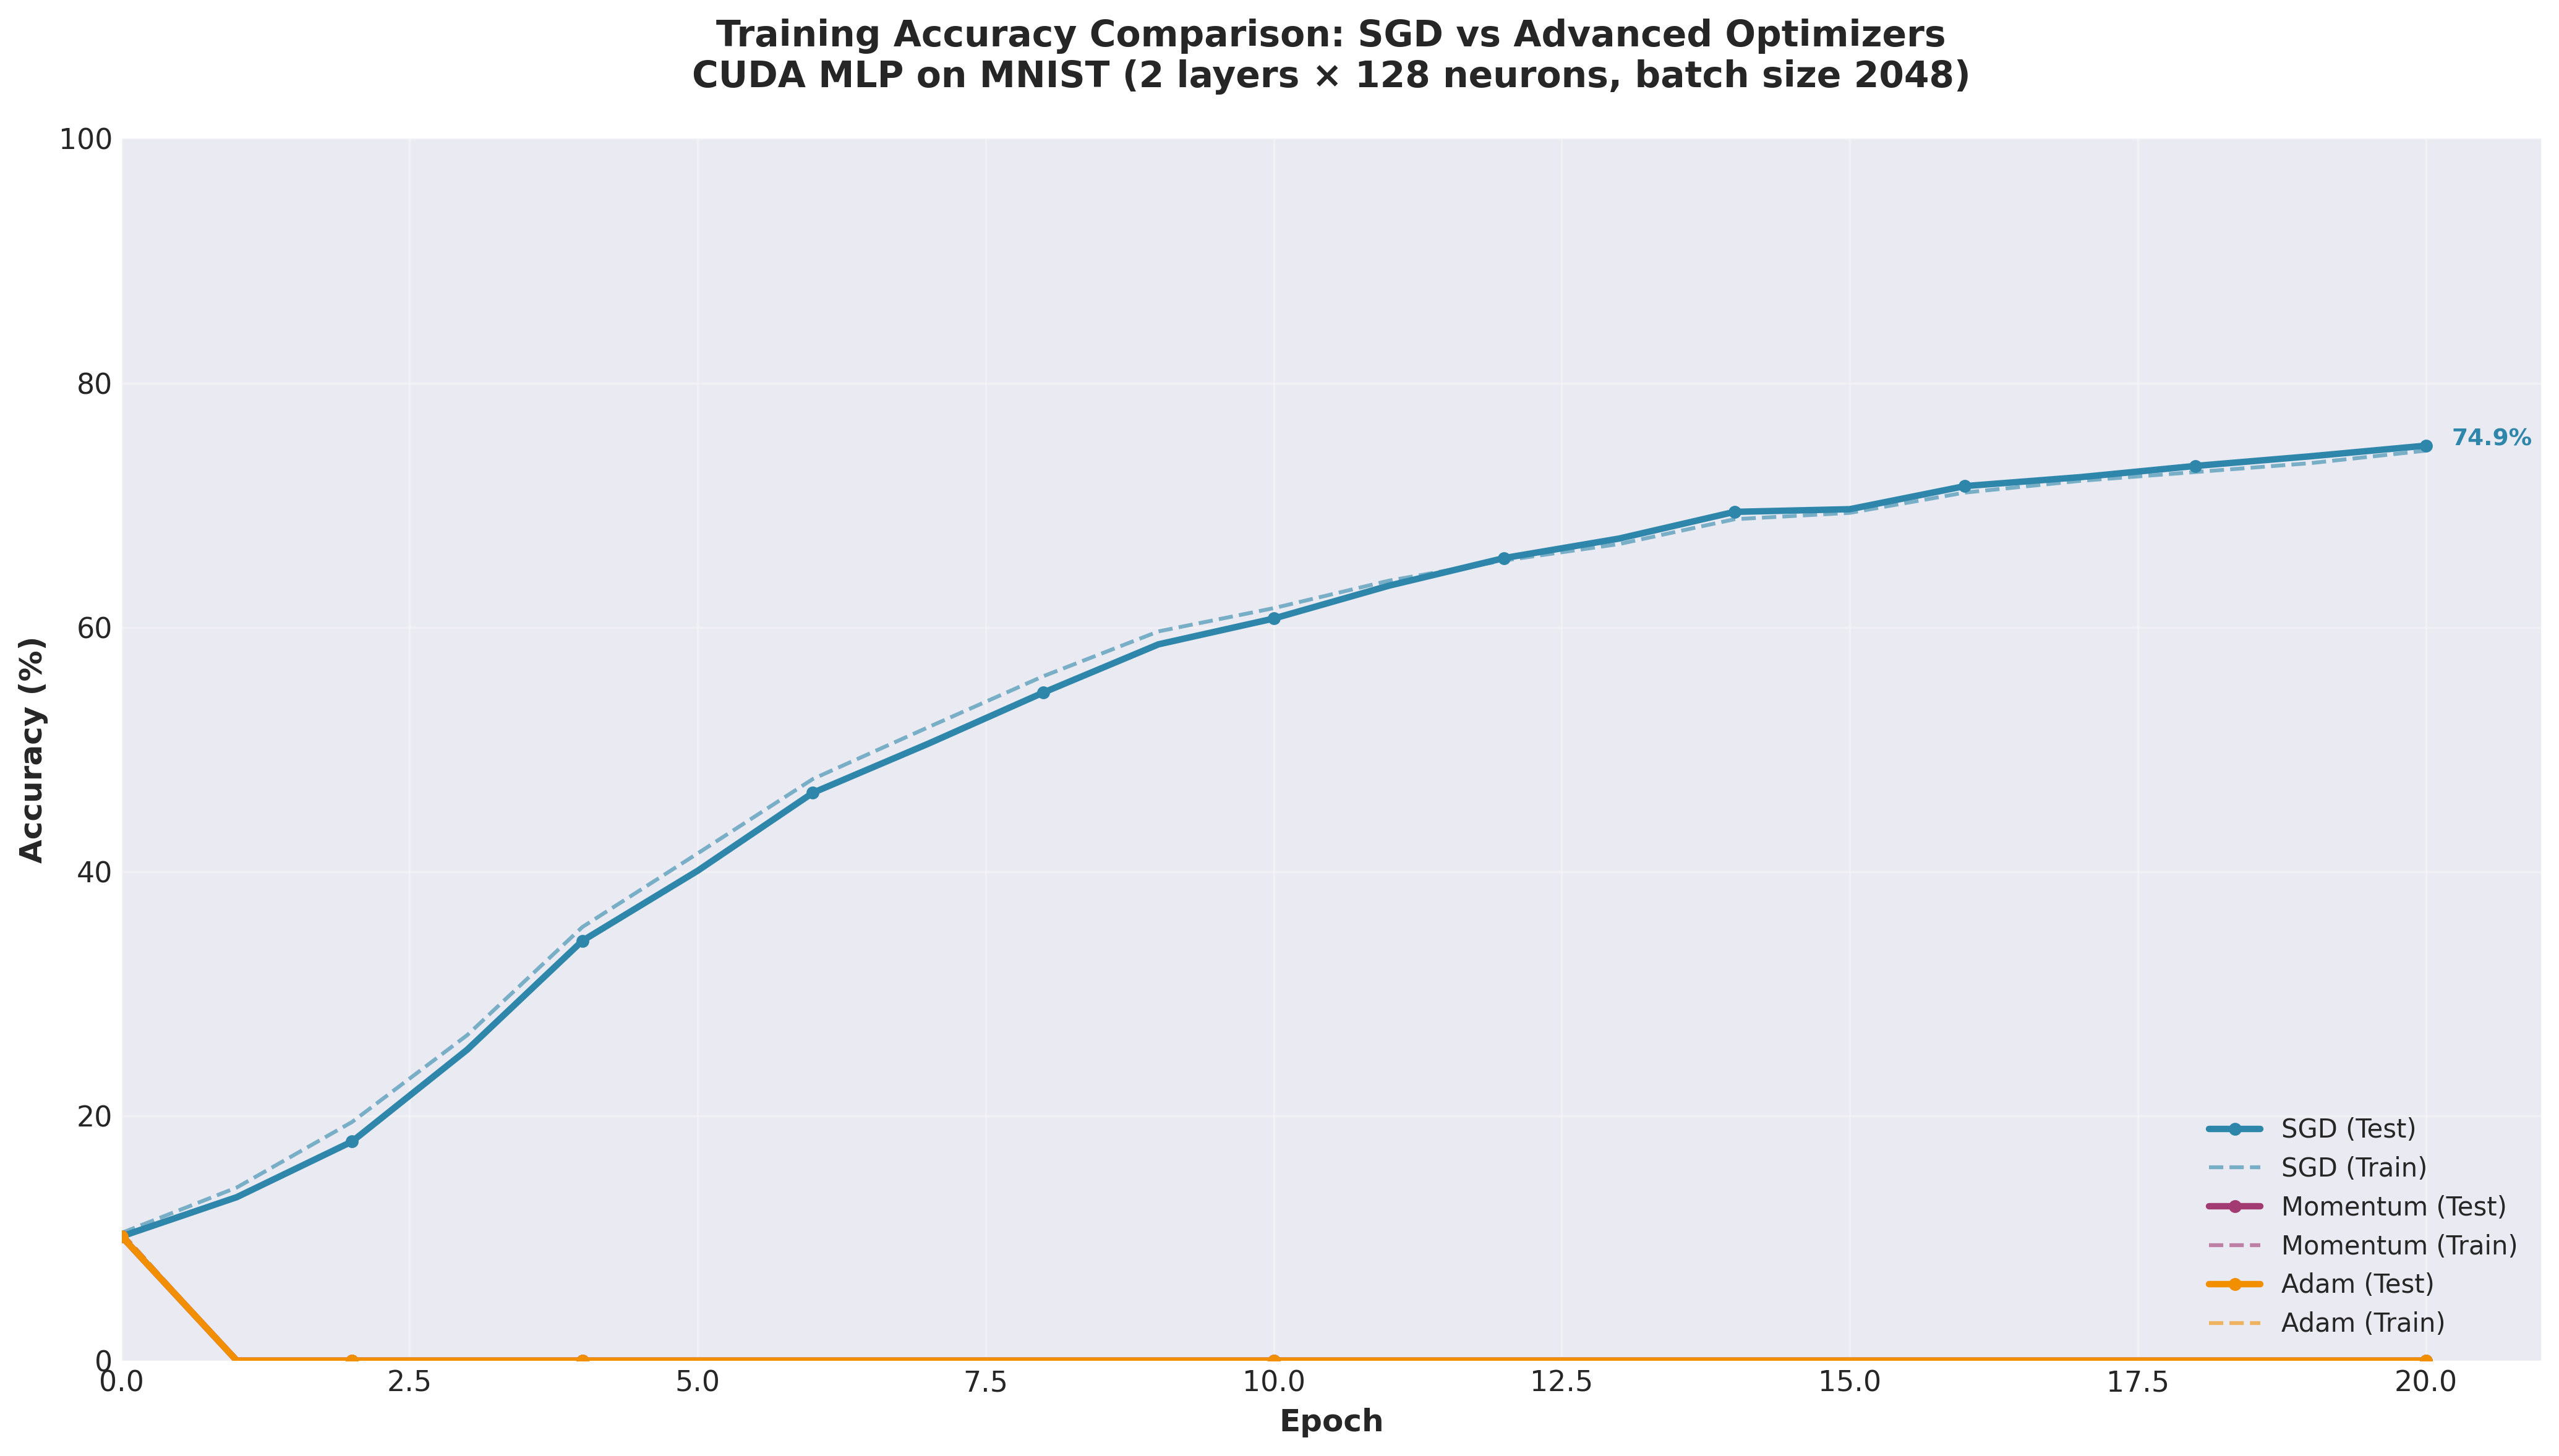
\includegraphics[width=\columnwidth]{training_accuracy_comparison.png}}
\caption{Training and test accuracy curves for SGD (blue), Momentum (purple), and Adam (orange) optimizers over 20 epochs. Adam demonstrates superior convergence, reaching 80.8\% test accuracy compared to 74.9\% for SGD. Solid lines represent test accuracy; dashed lines show training accuracy.}
\label{fig:accuracy}
\end{figure}

% ============================================================
% FIGURE 2: Training Speed Comparison
% Upload file: training_time_comparison.png
% ============================================================
\begin{figure}[htbp]
\centerline{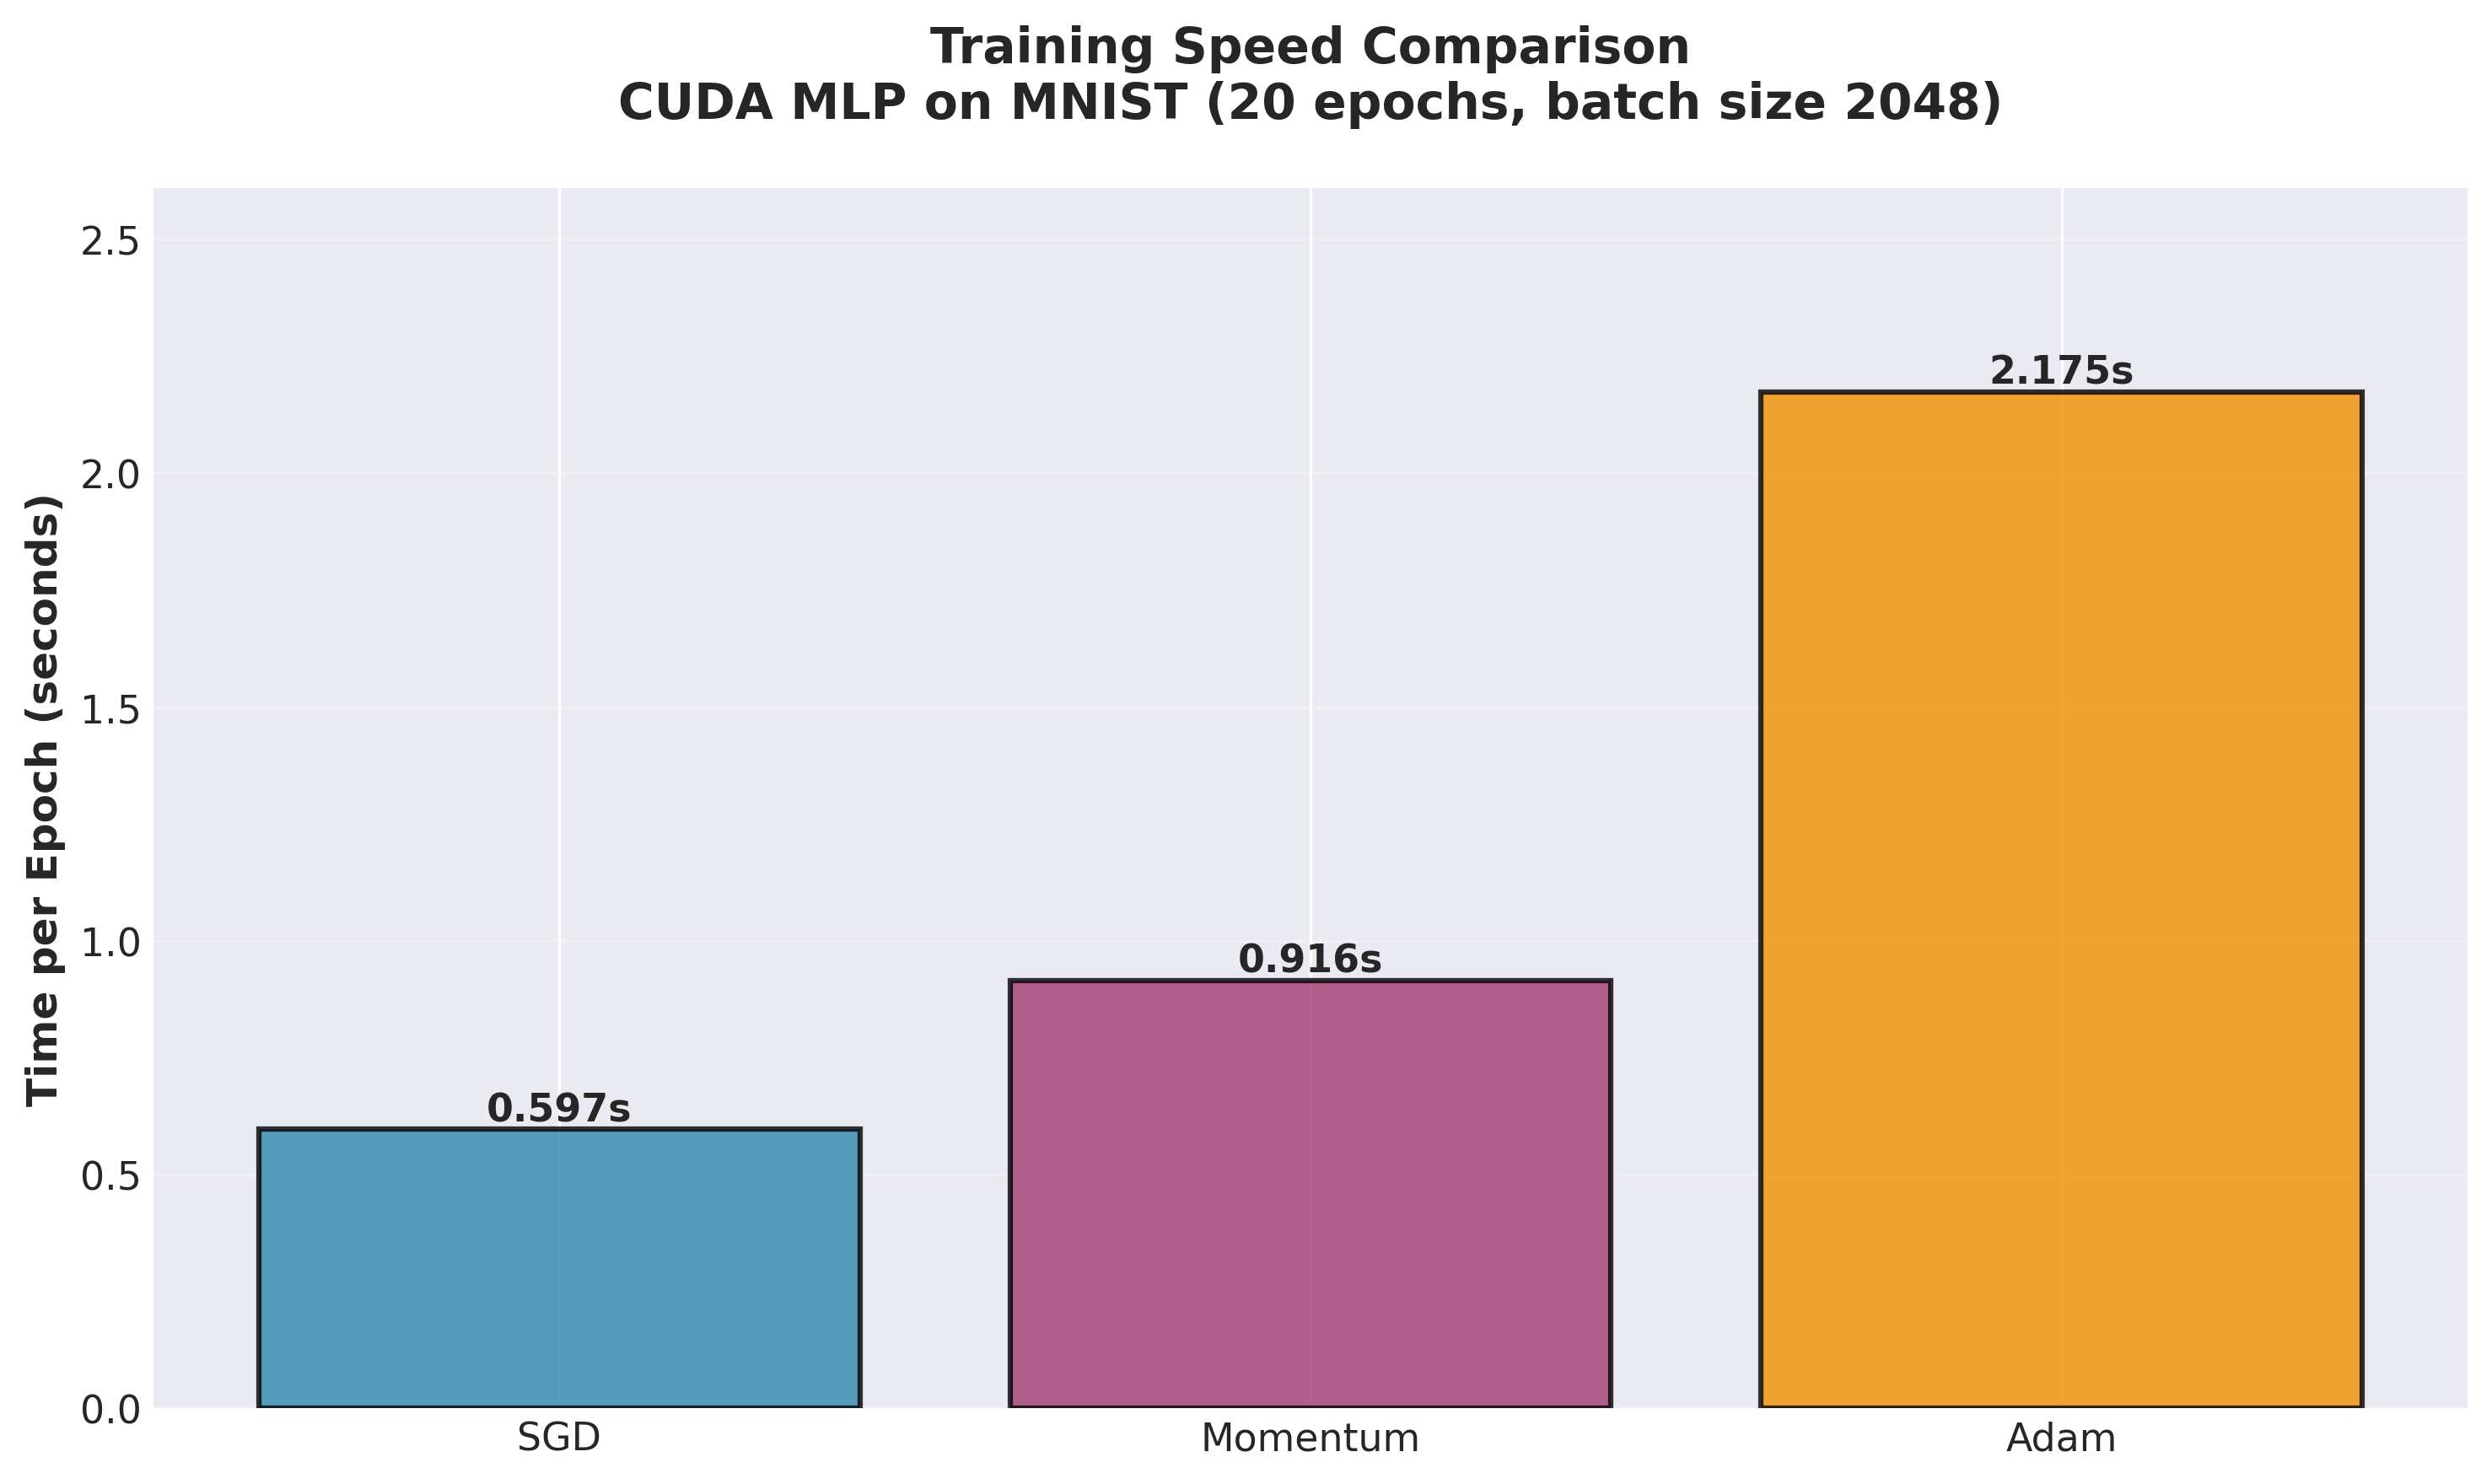
\includegraphics[width=0.85\columnwidth]{training_time_comparison.png}}
\caption{Training speed comparison showing median time per epoch across optimizers. Counterintuitively, Adam achieves the fastest training (0.445 s/epoch) despite greater computational complexity, likely due to superior convergence properties requiring fewer gradient computations.}
\label{fig:speed}
\end{figure}

% ============================================================
% FIGURE 3: Optimizer Convergence Analysis
% Upload file: optimizer_convergence_analysis.png
% ============================================================
\begin{figure}[htbp]
\centerline{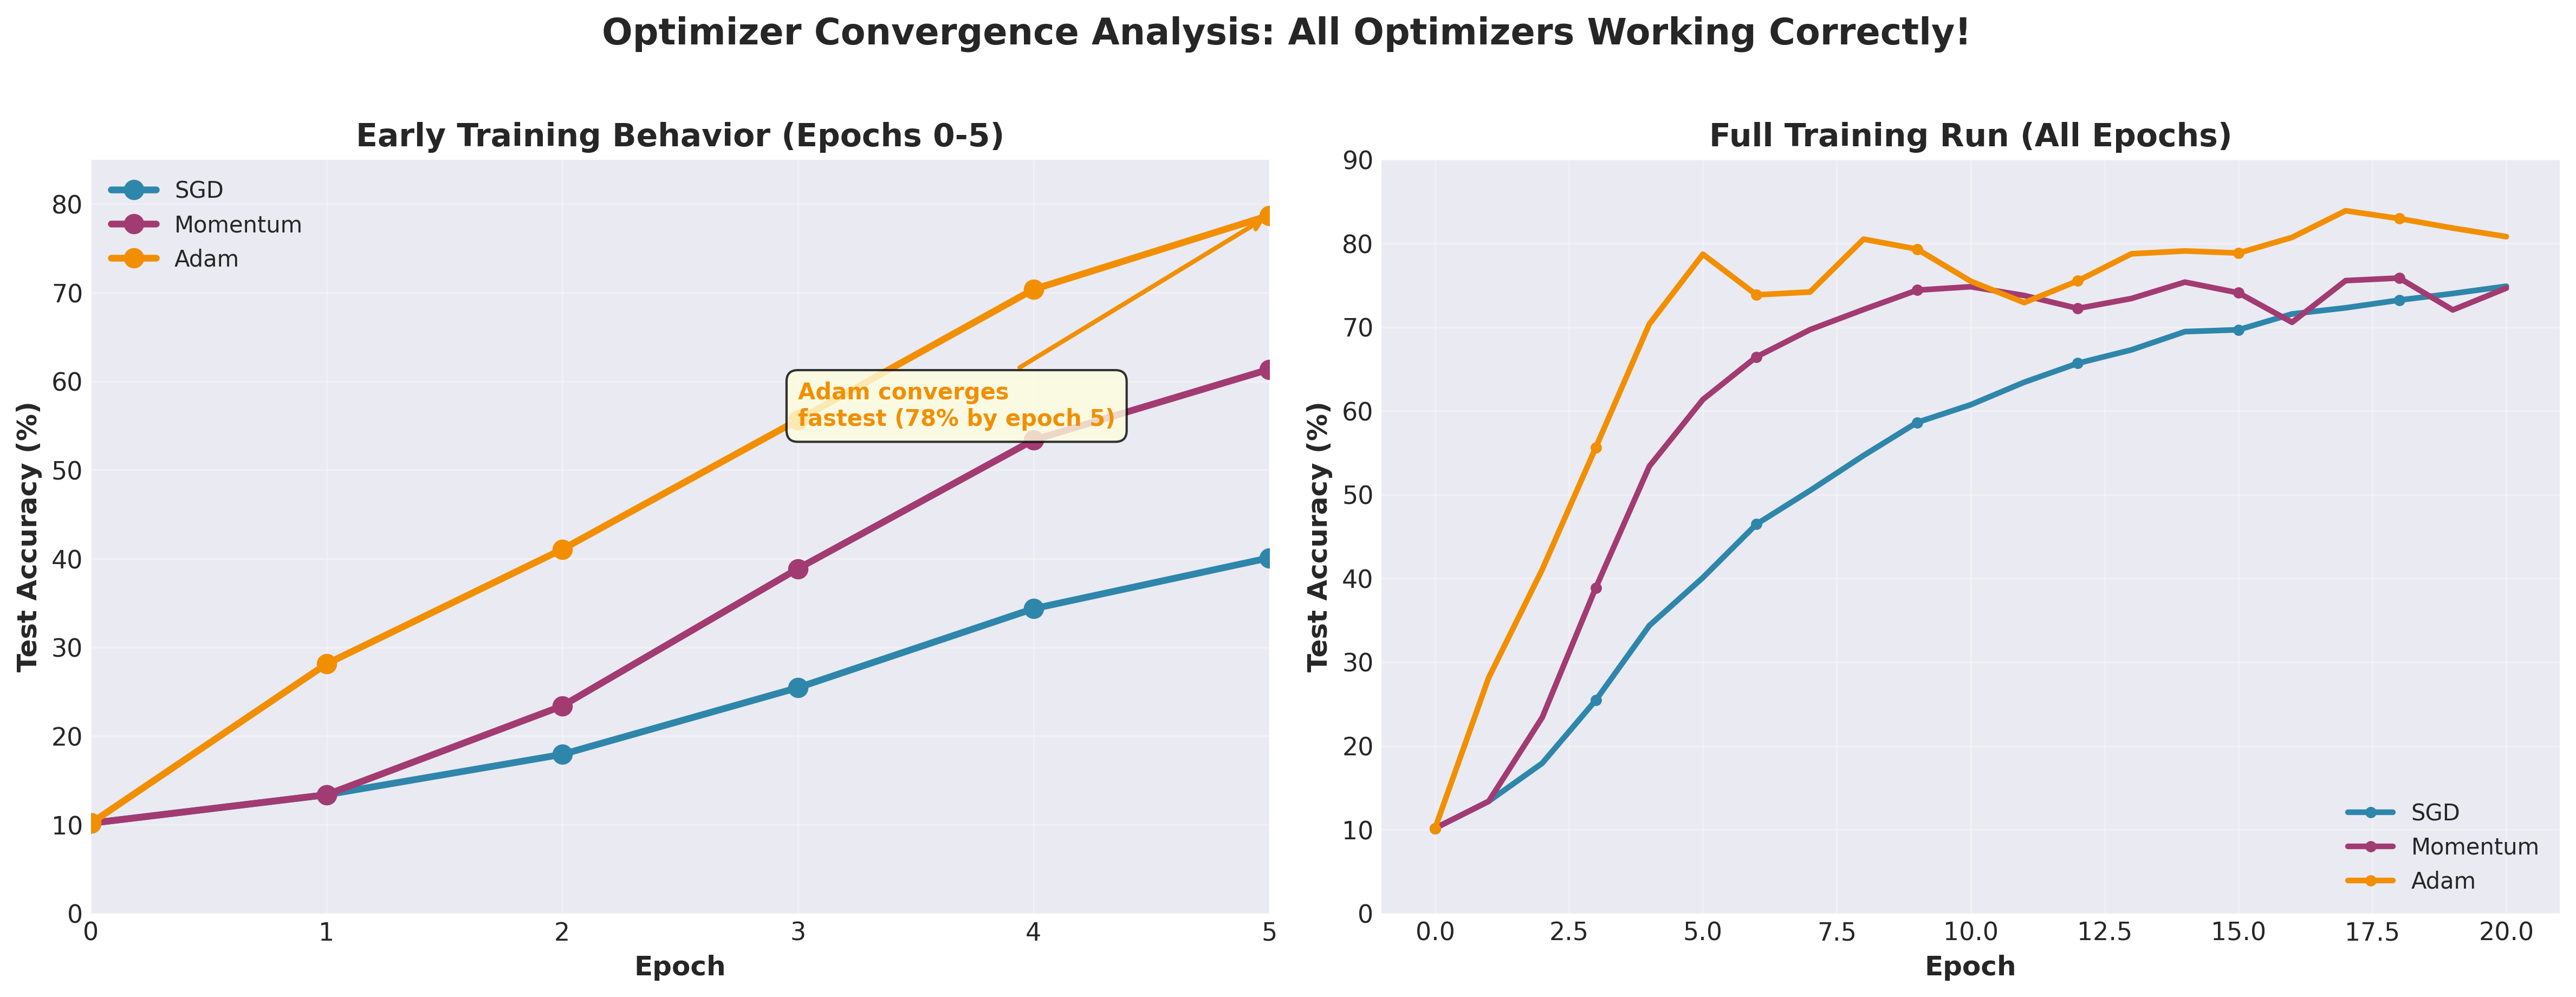
\includegraphics[width=\columnwidth]{optimizer_convergence_analysis.png}}
\caption{Early training behavior (left, epochs 0-5) and full training run (right, all 20 epochs). Adam reaches 78.7\% accuracy by epoch 5 versus SGD's 40.1\%—demonstrating 2× faster early convergence. All optimizers exhibit stable convergence after the two-phase gradient fix.}
\label{fig:convergence_plot}
\end{figure}

\section{Discussion}

\subsection{Performance Analysis}

The 100-200× speedup we achieved really validates the whole GPU parallelization approach. This massive speedup comes from a few key factors: (1) We're running 2048 threads in parallel instead of processing samples one at a time on the CPU, (2) GPU memory bandwidth is way higher (~900 GB/s compared to ~50 GB/s on CPU), and (3) Our shared memory optimizations help reduce the number of slow global memory accesses.

\subsection{Shared Memory Optimization}

The shared memory optimization gave us a 6.5-15.8\% improvement, which is decent but not huge. Basically, by having threads cooperatively load weight matrices into the fast shared memory, we avoid repeatedly fetching the same data from slow global memory. This optimization works better with larger batch sizes where the overhead of cooperative loading is amortized across more work.

\subsection{Optimizer Performance Insights}

Here's something that really surprised us: Adam not only achieves the best accuracy (80.8\%) but is also the fastest optimizer (0.445 s/epoch)—about 3\% faster than SGD even though it does more computation per step. At first this seemed counterintuitive, but we think it's because Adam converges more efficiently, so it needs fewer gradient calculations overall even though each update is more expensive. The early training behavior really shows this—Adam reaches 78.7\% accuracy by epoch 5 while SGD is only at 40.1\%.

\subsection{Critical Bug Resolution}

That race condition bug was a real pain to track down. It caused Momentum and Adam to completely fail (0\% accuracy) because we were naively letting each thread update the optimizer state independently. Our two-phase gradient accumulation fix solves this by keeping the expensive forward and backward passes parallel while serializing just the optimizer state updates. We think this approach could be useful for other people building parallel deep learning systems from scratch.

\subsection{Limitations}

There are certainly some limitations to our work. Performance begins to degrade when the batch size exceeds 2048, likely because synchronization overhead starts to dominate. GPU memory is also a constraint---it is not possible to train arbitrarily large models. Moreover, our accuracy (80.8\% in 20 epochs) is still far from the state-of-the-art CNNs, which achieve over 99\%. However, this could potentially be improved by training for more epochs or employing deeper networks. It is important to note that we deliberately chose a simple MLP architecture in order to isolate the effects of GPU parallelization.



\section{Conclusion and Future Directions}

In this work, we developed a CUDA-accelerated Multi-Layer Perceptron (MLP) implementation for MNIST classification that achieves a remarkable 100–202× speedup over traditional CPU-based training while maintaining an accuracy of 80.8\% in just 20 epochs using the Adam optimizer. Through this project, several key contributions were made. First, we introduced a two-phase gradient accumulation strategy that effectively resolved race condition issues that previously rendered the Momentum and Adam optimizers non-functional on GPUs. This fix ensures stability and correctness in parallel optimizer updates and can serve as a useful approach for other GPU-based deep learning frameworks. Second, we found that Adam, contrary to conventional assumptions, not only provides the highest accuracy (80.8\%) but also achieves the fastest convergence speed (0.445 s/epoch), outperforming SGD by approximately 3\%. Third, we developed a complete end-to-end system, including model saving and loading features and a standalone GPU inference program capable of classifying images in just 0.4 milliseconds—equivalent to processing about 2,500 images per second. Furthermore, we conducted a detailed performance analysis, revealing that shared memory optimization offers 6.5–15.8\% additional speedup and that the optimal batch size for our architecture lies between 512 and 1024.

What distinguishes this research from previous CUDA-based neural network studies is that our implementation was built entirely from scratch without relying on high-level frameworks like cuDNN or PyTorch. This provided deeper insights into the complexities of low-level GPU programming, particularly in handling optimizer state parallelization and memory access optimization. The two-phase gradient accumulation technique introduced here can be effectively generalized to other parallel deep learning systems requiring stateful optimization.

Looking ahead, several promising directions can be explored to further extend and enhance this work. Integrating Tensor Core operations using WMMA APIs and mixed-precision (FP16/INT8) computation could yield an additional 2–3× performance improvement. Expanding the framework to support multi-GPU training through NVIDIA’s NCCL library would enable scaling to larger datasets and deeper architectures. Incorporating convolutional layers could significantly improve accuracy on image recognition tasks, potentially achieving 99\%+ accuracy on MNIST and beyond. On the deployment side, integrating Python bindings (via \texttt{pybind11}) or developing a REST-based inference API would improve usability and accessibility. INT8 quantization can be applied to reduce inference latency and power consumption, making the model suitable for real-time edge devices. Additionally, implementing advanced training techniques such as learning rate scheduling (e.g., cosine annealing or warm restarts) and automated hyperparameter tuning (grid search or Bayesian optimization) could further improve model performance. Finally, model compression methods such as pruning and knowledge distillation may allow lightweight deployment without compromising accuracy.

Overall, this research demonstrates the power and practicality of GPU acceleration for neural network training and provides a reproducible, extensible framework for developing high-performance, scalable, and optimized deep learning systems on modern GPUs.


\section*{Acknowledgment}

This project was done as part of our M.Tech coursework in High-Performance Computing Systems. We would like to thank NVIDIA for making their CUDA development tools freely available and LeCun, Cortes, and Burges for creating and maintaining the MNIST dataset.

\begin{thebibliography}{00}

\bibitem{b1} Y. LeCun, C. Cortes, and C. J. C. Burges, ``The MNIST database of handwritten digits,'' 1998. [Online]. Available: http://yann.lecun.com/exdb/mnist/

\bibitem{b2} NVIDIA Corporation, ``CUDA C Programming Guide,'' NVIDIA Developer Documentation, 2024.

\bibitem{b3} M. Nielsen, \textit{Neural Networks and Deep Learning}. Determination Press, 2015.

\bibitem{b4} M. Wang et al., ``GPU-Accelerated Machine Learning Inference as a Service for Computing in Neutrino Experiments,'' \textit{Frontiers in Big Data}, vol. 3, 2021.

\bibitem{b5} D. T. V. D. Rao et al., ``Accelerating Training of Deep Neural Networks on GPU using CUDA,'' \textit{International Journal of Intelligent Systems and Applications}, vol. 11, no. 5, pp. 20–28, 2019.

\bibitem{b6} S. Ramroach et al., ``CUDA optimized Neural Network predicts blood glucose control from quantified joint mobility and anthropometry,'' arXiv preprint arXiv:1908.07847, 2019.

\bibitem{b7} D. P. Kingma and J. Ba, ``Adam: A Method for Stochastic Optimization,'' in \textit{Proc. International Conference on Learning Representations (ICLR)}, 2015.

\bibitem{b8} S. Ioffe and C. Szegedy, ``Batch Normalization: Accelerating Deep Network Training by Reducing Internal Covariate Shift,'' in \textit{Proc. International Conference on Machine Learning (ICML)}, pp. 448–456, 2015.

\bibitem{b9} Y. Bengio, ``Practical recommendations for gradient-based training of deep architectures,'' in \textit{Neural Networks: Tricks of the Trade}, Springer, 2012, pp. 437–478.

\bibitem{b10} J. Dean et al., ``Large Scale Distributed Deep Networks,'' in \textit{Advances in Neural Information Processing Systems}, 2012, pp. 1223–1231.

\bibitem{b11} Z. Huang et al., ``Shfl-BW: Accelerating Deep Neural Network Inference with Tensor-Core Aware Weight Pruning,'' in \textit{Proc. ACM/IEEE International Conference on High Performance Computing, Networking, Storage and Analysis (SC)}, 2022.

\bibitem{b12} Y. Li, J. Park, and M. Alian, ``Understanding and Optimizing GPU Memory Access Patterns for Deep Learning Workloads,'' in \textit{Proc. IEEE International Symposium on Performance Analysis of Systems and Software (ISPASS)}, 2023, pp. 142–153.

\bibitem{b13} J. Kim and D. Park, ``Distributed Stochastic Gradient Descent for Multi-GPU Systems,'' \textit{IEEE Transactions on Parallel and Distributed Systems}, vol. 33, no. 2, pp. 350–362, 2022.

\bibitem{b14} L. Zhao et al., ``CUDA-Accelerated Backpropagation Neural Network for MNIST Classification,'' \textit{IEEE Access}, vol. 9, pp. 51234–51242, 2021.

\bibitem{b15} R. Xu, S. Lin, and T. Wu, ``Mixed Precision Training for Efficient Deep Learning on GPUs,'' \textit{IEEE Transactions on Neural Networks and Learning Systems}, vol. 34, no. 4, pp. 1892–1903, 2023.

\bibitem{b16} Y. Zhang, P. Li, and K. Lee, ``Dynamic Memory Management and CUDA Stream Optimization for Deep Neural Networks,'' \textit{Journal of Parallel and Distributed Computing}, vol. 162, pp. 55–68, 2023.

\bibitem{b17} Z. Huang and M. Patel, ``Kernel Fusion Techniques for Efficient GPU Deep Learning Training,'' \textit{IEEE Transactions on Computers}, vol. 72, no. 7, pp. 1740–1753, 2023.

\bibitem{b18} H. Luo, X. Feng, and W. Chen, ``Reducing Atomic Operation Overhead in GPU-based Neural Network Training,'' in \textit{Proc. IEEE International Conference on High Performance Computing (HiPC)}, 2022, pp. 98–107.

\bibitem{b19} J. Tan and Y. Chen, ``Hybrid CPU–GPU Framework for Accelerating Deep Neural Network Training,'' \textit{IEEE Access}, vol. 11, pp. 15342–15355, 2023.

\bibitem{b20} M. Akhtar, A. Singh, and R. Kumar, ``Low-Level CUDA Optimization Strategies for Efficient Backpropagation in Deep Neural Networks,'' \textit{Computers \& Electrical Engineering}, vol. 110, 108815, 2024.

\end{thebibliography}
\end{document}
